\documentclass[a4paper,10pt,notitlepage]{article}
\usepackage[utf8]{inputenc}
\usepackage{fullpage}
\usepackage{amsmath,amsthm,amssymb}
\usepackage{url}
\usepackage{hyperref}
\usepackage{listings}
\usepackage[usenames,dvipsnames]{color}
\usepackage[stable]{footmisc}
\usepackage{caption}
\usepackage{hyphenat}
\usepackage{courier}
\usepackage{graphicx}
\DeclareCaptionFont{white}{\color{white}}
\DeclareCaptionFormat{listing}{\colorbox{Gray}{\parbox{\textwidth}{#1#2#3}}}
\captionsetup[lstlisting]{format=listing,labelfont=white,textfont=white}
\definecolor{lightgray}{gray}{0.9}
\graphicspath{{./images/}}

\lstset{
	language=C,
	basicstyle=\small\ttfamily,
	commentstyle=\color{Gray},
	tabsize=4,
	numbers=left,
	numberstyle=\tiny,
	stepnumber=1,
	numbersep=5pt,
	backgroundcolor=\color{lightgray},
	}

\title{Parallel Algorithms and Parallel Computers (IN4026) \\ Lab report}
\author{Źmicier Žaleźničenka (4134575) \\ \\
D.V.Zhaleznichenka@student.tudelft.nl}
\date{\today}

\begin{document}

\maketitle

\section{Prefix/suffix minima problem}

\subsection{Introduction}

In the first assignment it was required to devise an efficient algorithm computing prefix and suffix minimas for the given array\footnote{Given an array \(A = (a_1, . . . , a_N)\) with elements drawn from a linear ordered set. The suffix minima problem is to determine \(min\{a_i, a_{i+1}, . . . a_N\}\) for each $i$. The prefix minima are \(min\{a_1, a_2, . . . a_i\}\) for each $i$.}. 

Despite it is easy to compute prefix/suffix minimas sequentially with \(T = O(N)\), it was required to find an algorithm that would have better performance in the parallel setup as the performance of the sequential solution for the large data sets is not satisfactory.

The algorithm idea was found at Wikipedia page explaining prefix sums\footnote{$http://en.wikipedia.org/wiki/Prefix\_sum$}. The algorithm is recursive and consists of three steps. First of all, we compute the minimas of consecutive pairs of items in which the first item of the pair has an even index and store them in a separate array. Secondly, we recursively compute the minimas for the obtained array. At the last step, we expand the computed sequence with the help of the source array. Here, each element is either directly copied from the previously computed sequence or is calculated using the element in the source array and a partial minima from the previously computed sequence. The first and the third steps in this algorithm can be parallelized easily. The second step of the algorithm is the recursive call that eventually expands into a series of the first and the third steps, thus not being a bottleneck of the algorithm. 

\subsection{Algorithm proof}

The recursion is performed in two steps. In the first step for several times we discard from the original sequence half of its elements. We do it in such a way that all the remaining elements are the least in the consequent element pairs of the source seqence. We reduce the sequence until only one element remains in it. By design, this element is the minima of the sequence. 

After we find the minimal element, we expand the sequence back. At each recursion step up to the original sequence for each element in the source sequence we get a local minima, i.e. the minima of preceeding sequence (for prefix minima problem) or the minima of the subsequent sequence (for suffix minima problem). To find out the element that should be placed in a prefix/suffix minima sequence instead of the original element, we compare the original element with the local minima and select the smallest element for odd values or just take the local minima for the even values, as the local minima already concerns the original element in this case. 

\subsection{Time-complexity analysis}

The time-work calculations here were done for the prefix minima problem. The computational complexity of the suffix minima problem is the same.

\begin{lstlisting}

//prefix(A, N) - find prefix minima for array A of size N
//input:  array A[0..N-1]
//output: array B[0..N-1] array of prefix minimas for A

1.  for 0 < i < N pardo //W = O(N), T = O(1)
		if i is even then Z[i/2] = min(A[i],A[i+1])

2.  Z = prefix(Z, N/2)		//W = W(N/2), T = T(N/2)

3.  for 1 < i < N pardo //W = O(N), T = O(1)
		if i is odd then B[i] = Z[i/2]
		else B[i] = min(A[i], Z[i/2-1])

//T(N) = T(N/2) + O(1) = O(log n)
//W(N) = W(N/2) + O(N) = O(N)		
	
\end{lstlisting}

\subsection{Implementation}

The algorithm reads source data from the file. The output of the results is suppressed but it can be enabled with the help of the preprocessor directive. The algorithm was tested with the sequence suggested in the task description (file base.test), increasing sequence (inc.test) and decreasing sequence (dec.test). To do the performance tests described in the following section, three generated test files were used. They contained 262144, 524288 and 1048576 elements. The data generator is written in Python and can be found in datagen.py file. After performing the initial performance testing, it was decided to work with the biggest test file as it demonstrates the effect of parallelizing the algorithm in the best way. For the smaller data sets it turned out that the overhead of threading operations and/or noise from the other OS tasks does not allow to retrieve reliable results.

The sequential implementation of the algorithm is straightforward and is based on pseudocode provided in the previous section. The function \lstinline{scan_seq()} accepts the source array, its length and prefix value as the parameters. The prefix value is needed to distinguish between prefix and suffix minima computations. 

The sequential implementation contains three OpenMP directives needed to parallelize the work-intensive parts of the algorithm. To parallelize the first step of the algorithm we need in one pragma and to parallelilize the third step we use two pragmas, one for prefix computations and one for suffix computations. All the pragmas have the following structure.

\begin{lstlisting}
#pragma omp parallel for \
	shared (Z, source, chunk, num_threads) private (i) \
	schedule (static, chunk) \
	num_threads (num_threads)
\end{lstlisting}

In each round of computations, \lstinline{scan_seq()} function is invoked twice, once for prefix computations and once for suffix computations. Though it is possible to compute both prefixes and suffixes in one round we have decided to split the computations as according to the requirements both resulting arrays should be stored in array $B$. Thus, we have to reinitialize array $B$ between the computations. This is done in the function \lstinline{seq_function()}. While doing performance tests, we measure the execution time of this function.

The threaded version of the algorithm is organized the same way. We have a function \lstinline{par_function()} that calls \lstinline{scan_par()} function twice and reinitializes $B$ in between. All the computations are performed in \lstinline{scan_par()} function. 

We have rewritten the code of \lstinline{main()} function to move the pthreads-related code from it to \lstinline{scan_par()} function. We think that our implementation of the threaded version required such a change. 

As we did it with the OpenMP part, we have parallelized the first and the third steps of the algorithm. The first step is implemented in function \lstinline{par_sum()}, the third is implemented in function \lstinline{par_odd}. At each recursion step, we create the required number of threads in the main thread executing the code of \lstinline{scan_par()} function, wait for the completion of the first step, destroy the threads and go deeper. When the recursion is over and we get back, we create the new threads, wait for the completion of the third step and destroy the threads. Here, we stick to the boss-worker threading model.

With this solution, we have an additional overhead due to the need to create and destroy the worker threads in each recursion step. It would make more sense to create the threads pool only once and feed them with the new parameters when needed. However, we were not able to implement the thread pool correctly with pthreads framework.

In our solution, at each recursion step, the problem space is divided into subspaces that are assigned to the worker threads. Each thread computes a fixed amount of $N/nrT$ values. The subspaces do not overlap, thus it is safe for the threads to read and write needed values concurrently.

There were introduced two optimizations. First, we tried to optimize the creation of threads by limiting their number for non-intensive operations. At the last steps of recursion, when there are only several values to compute, it is cheaper not to create many threads for this task, but to assign all the tasks to one thread only, or to a small number of threads. The logic of this improvement is implemented in \lstinline{get_optimal_threads_number()} function. It turned out that this optimization may lead to the significant performance improvement for the large data sets and many threads\footnote{I.e., execution time was decreased by approximately 25\% for 1m elements and 8 threads.}. Also, this optimization was helpful as we needed to limit the number of threads for the situations with less values than threads. However, to have more descriptive results that would better show the performance differences of the setups with different number of threads, this optimization was only used not to allow to create more threads than remaining elements.

Secondly, we had to optimize the process of initializing the source array. We started to test the program with large auto-generated arrays and it turned out that we cannot trust the performance results as prefix/suffix minimas for such arrays become degenerated soon. To mitigate this problem, in the rewritten initialization function we implicitly put the smallest value to the end of sequence for prefix minima computations and to the start of sequence for suffix minima. This ensures that during all the recursion steps all the threads will be busy doing actual computations. Advanced initialization can be switched off with the help of the preprocessor directive and it has to be switched off to use small data sets as the test files were not updated to correspond with this sort of initialization procedure.

\subsection{Tests}

The performance tests were done at the 8-core university server\footnote{exp02.st.ewi.tudelft.nl}.

We have executed the performance tests for several times to see whether the results are stable. It turned out that in some of the runs there were anomalies (for one or two values the execution time was bigger than expected) that could be caused by the OS overhead. However, the most runs gave us similar results. We have taken two stable samples, one testing execution time and one testing speedup to build the performance charts. The samples are provided in tables 1-2, the charts can be found in figures 1-4.

\begin{table}[!htb]
  \centering
  \begin{tabular}{ | c | c | c | c | c | c | c | c | }
  \hline
NSize &	Iter & Sequential & Th01 & Th02 & Th04 & Th08 & Par16 \\ \hline  
16384 & 10 & 0.010149 & 0.020914 & 0.021119 & 0.038229 & 0.081349 & 0.154972 \\ \hline
32768 & 10 & 0.020040 & 0.032029 & 0.028222 & 0.045403 & 0.088974 & 0.170114 \\ \hline
65536 & 10 & 0.040165 & 0.053762 & 0.041644 & 0.056487 & 0.098804 & 0.187677 \\ \hline
131072 & 10 & 0.080324 & 0.096686 & 0.065299 & 0.078095 & 0.114957 & 0.207896 \\ \hline
262144 & 10 & 0.159584 & 0.188526 & 0.115658 & 0.120709 & 0.184255 & 0.291002 \\ \hline
524288 & 10 & 0.320757 & 0.356628 & 0.213272 & 0.197545 & 0.209603 & 0.334386 \\ \hline
1048576 & 10 & 0.661932 & 0.704599 & 0.410030 & 0.353673 & 0.308857 & 0.418124 \\ \hline
  \end{tabular}
  \caption{Time execution test}
  \end{table}

\begin{table}[!htb]
  \centering
  \begin{tabular}{ | c | c | c | c | c | c | c | c | }
  \hline
 NSize & Iter & Sequential & Th01 & Th02 & Th04 & Th08 & Par16 \\ \hline  
16384 & 10 & 0.011346 & 0.483323 & 0.480213 & 0.257448 & 0.121707 & 0.058737 \\ \hline  
32768 & 10 & 0.019488 & 0.524633 & 0.657468 & 0.392365 & 0.196001 & 0.102196 \\ \hline  
65536 & 10 & 0.038948 & 0.637718 & 0.883535 & 0.640045 & 0.357814 & 0.188464 \\ \hline  
131072 & 10 & 0.077692 & 0.717411 & 0.970992 & 0.658691 & 0.519224 & 0.314279 \\ \hline  
262144 & 10 & 0.155364 & 0.767704 & 1.241690 & 1.269967 & 1.021950 & 0.556715 \\ \hline  
524288 & 10 & 0.310239 & 0.806700 & 1.387281 & 1.526737 & 1.528113 & 1.01387 \\ \hline  
1048576 & 10 & 0.620419 & 0.800950 & 1.417948 & 1.722917 & 2.059222 & 1.329659 \\ \hline  
  \end{tabular}
  \caption{Speedup execution test}
  \end{table}

\begin{figure}[!htb]
\centering
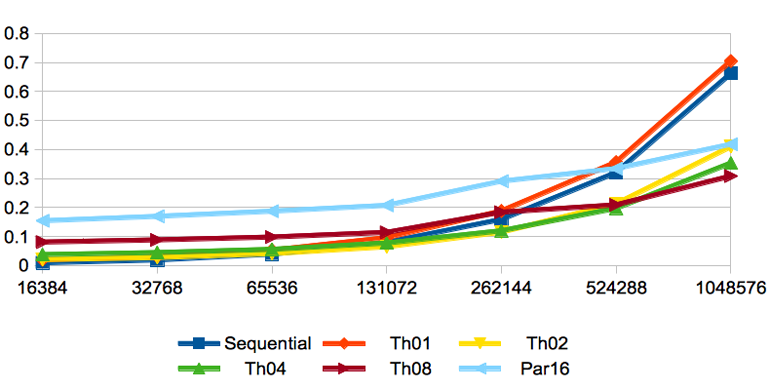
\includegraphics[scale=0.5]{1-tn.png}
\caption{T(N, P fixed) chart}
\label{fig:1-tn}
\end{figure}

\begin{figure}[!htb]
\centering
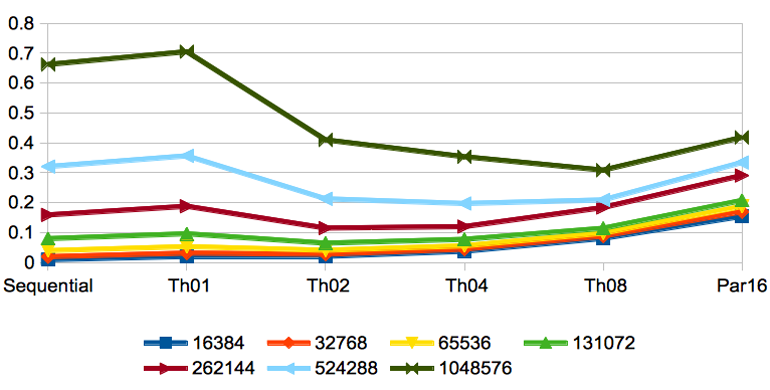
\includegraphics[scale=0.5]{1-tp.png}
\caption{T(P, N fixed) chart}
\label{fig:1-tp}
\end{figure}

\begin{figure}[!htb]
\centering
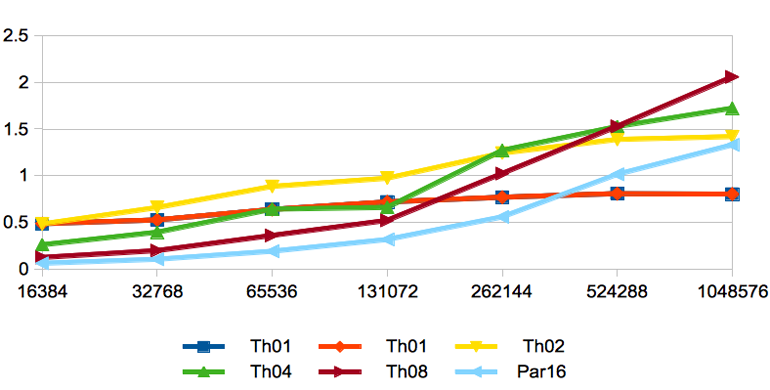
\includegraphics[scale=0.5]{1-sn.png}
\caption{Speedup(N, P fixed) chart}
\label{fig:1-sn}
\end{figure}

\begin{figure}[!htb]
\centering
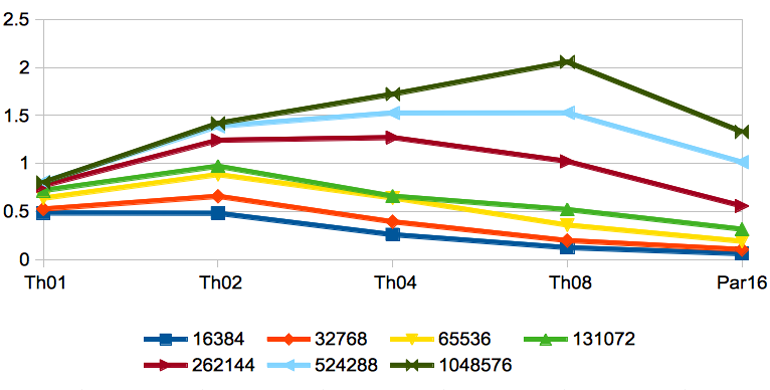
\includegraphics[scale=0.5]{1-sp.png}
\caption{Speedup(P, N fixed) chart}
\label{fig:1-sp}
\end{figure}

From the analysis of the performance charts we can state the following. First of all, we see that the algorithm is indeed multi-threaded, and the more processing cores we have, the better is algorithm performance, both in terms of execution time and speedup. The more sample data we have, the better we see the difference in execution times between different numbers of employed processor cores. For the small samples the difference between the number of used threads is minimal due to the threading code/OS tasks overhead.

At \autoref{fig:1-tn} we see that the slope of single-threaded and sequential runs is much steeper than for the multi-threaded runs. We observe this because the time difference between single-threaded runs and multi-threaded runs increases with the increase of the number of samples. We also see that 16-threaded run is less efficient than any other multi-threaded run. This is because we have only eight cores available and if we use 16 threads, they are used inefficiently and much time is spent to switch between the threads in the processor cores. However, the more samples we have, the better performance is observed for 16-threads run. We can predict that if we have even more samples, the performance of 16-threads run will end up between 4-threads and 8-threads runs as this overhead will play smaller role for large setups. Also, at \autoref{fig:1-tn} we see that the performance of 8-threads run is better than the performance of 4-threads run, and the performance of 4-threads run is better than the performance of 2-threads run, which is correct.

At \autoref{fig:1-tp} we see that for the largest sample we have performance improvements up to eight threads. For the second largest sample the performance of 8-threads and 4-threads runs is the same. For smaller samples the performance of 8-threads run is worse than the performance of 4-threads run. This is caused by the additional overhead of the threads creation and destruction. If we have more sample data, its performance chart should resemble the chart for the largest sample, as for the samples of this size the overhead doesn't play an important role anymore. From \autoref{fig:1-tp} we also see that the performance of single-thread soltion is worse than the performance of sequential solution, and the performance of 16-threads solution is worse than the performance of 8-threads solution, which is correct.

It is also interesting to compare the performances of the largest and the second largest samples. We see that the more threads we have, the less is the performance difference. For one and two threads it takes twice the time of the second largest sample to process the largest sample, for eight threads it takes only 1.5 times more time to process it if comparing with the second largest sample processing time.

The speedup charts confirm the conclusions drawn from the time charts. From \autoref{fig:1-sn} we see that the speedup for 8-threads run is the biggest. 4-threads and 2-threads runs also provide significant speedup for large samples. From \autoref{fig:1-sp} we see that the larger is the data set and the more employed cores we have, the better is the speedup. To find the speedup limit, we need in bigger samples.

\subsection{Conclusions}

In this exercise we have learnt the ways to parallelize the prefix sum problem and studied the ways to create multi-threaded programs in C programming language using OpenMP and pthreads libraries. Both of these libraries provide effective solutions to create multi-threaded programs, though pthreads allows to manage multi-threading in more advanced way. However, it is easier to parallelize C programs using OpenMP. C itself is a very efficient language for writing multi-threaded programs as it introduces low overhead and operates on low level. However, C is rather difficult for programmers as it doesn't have automatic memory management.

\section{Simple merge problem}

\subsection{Introduction}

\subsection{Algorithm proof}

\subsection{Time-complexity analysis}

\subsection{Implementation}

\subsection{Tests}

\subsection{Conclusions}


\section{List ranking (pointer jumping) problem}

\subsection{Introduction}

\subsection{Algorithm proof}

\subsection{Time-complexity analysis}

\subsection{Implementation}

\subsection{Tests}

\subsection{Conclusions}

\end{document}
